\documentclass[a4paper,11pt]{article}
\usepackage{sbpo-template}
\usepackage[brazil]{babel}
\usepackage[latin1]{inputenc}
\usepackage{amsmath,amssymb}
\usepackage{url}
\usepackage[square]{natbib}
\usepackage{indentfirst}
\usepackage{fancyhdr}
\usepackage{graphicx}

\pagestyle{fancy}
\fancyhf{}
\fancyhead[C]{
\includegraphics[width=\textwidth]{cabecalho_sbpo.png}}
\renewcommand{\headrulewidth}{0pt}
\setlength\headheight{101.0pt}
\addtolength{\textheight}{-101.0pt}
\setlength{\headsep}{-5mm}

\begin{document}

\title{Test-Assignment Problem} 

\maketitle
\thispagestyle{fancy}

\author{
\name{Murilo Antunes Goedert}
\institute{Engenharia de Software
UDESC}
\iaddress{Ibirama/SC - Brasil}
\email{murilogoedert@gmail.com}
}

\author{ 
\name{Victor Hugo Grabowski Beltramini}
\institute{Engenharia de Software
UDESC}
\iaddress{Ibirama/SC - Brasil}
\email {vhbeltramini@gmail.com}
}

\vspace{8mm}
\begin{resumo}
A atribui\c c\~ao de testes \'e um problema de otimiza\c c\~ao complexo, consiste em encontrar a melhor maneira de 
distribuir um conjunto de diferentes testes dentro de uma sala de aula a fim de minimizar a probabilidade de ocorrer cola. O presente documento tem como objetivo resolver esse problema de otimiza\c c\~ao implementando 
um conjunto de metaheur\'isticas incluindo estrat\'egias construtivas e por modifica\c c\~ao, e realizando um estudo experimental a partir do resultado 
destas implemeta\c c\~oes.
 \end{resumo}

\bigskip
\begin{palchaves}
Aloca\c c\~ao de testes, Metaheur\'isticas, Problemas de otimiza\c c\~ao.

\end{palchaves}


\vspace{8mm}

\begin{abstract}
The test assignment is a complex optimization problem, it consists of finding the
best way to distribute a set of different tests within a classroom in order to minimize
the probability of cheating occurring. This document aims to solve this problem
of optimization by implementing a set of meta-heuristics including constructive strategies and
by modification, and carrying out an experimental study from the result of these implementations.

\end{abstract}

\bigskip
\begin{keywords}
Test-Assignment. Metaheuristics. Optimization problems.

\end{keywords}

 
\newpage
\section{Introdu\c{c}\~ao} 
 
A partir do momento que temos a aplica\c c\~ao de um conjunto de testes em um grupo de concorrentes queremos eliminar ao m\'aximo a probabilidade de que possa ocorrer copia de respostas entre estes concorrentes 
pois isso estar\'a afetando o resultado final dos melhores classificados, a partir disso que surge o problema de aloca\c c\~ao de de testes. 
A probabilidade e facilidade de que se ocorra cola pode se dar a partir de alguns fatores,
sendo eles por exemplo a proximidade entre as carteiras e o qu\~ao similares s\~ao as provas. Sendo assim, par cada par de carteiras pode ser, a partir desses fatores, definido um fator de probabilidade de cola, que \'e o produto da dist\^ancia entre as carteiras e a similiaridade entre as provas aplicadas nestas.

Inicialmente podemos representar o problema usando grafos, cada v\'ertice sendo uma carteira e cada aresta definindo que as carteiras representadas pelos v\'ertices est\~ao contectadas no problema, ou seja, devem ser consideradas no resultado da fun\c c\~ao objetivo. Os dados do problema ent\~ao s\~ao: O conjuto de Testes T, o conjunto de carteiras D, a matriz de proximidades P e a matriz de sim\'ilaridades entre os testes Y, F o conjunto de carteiras que n\~ao possuem prova. Adicionalmente, como nem todas as carteiras encontram-se pr\'oximas o suficiente para serem consideradas, temos E como sendo o subconjunto de carteiras em D que est\~ao pr\'oximas. O problema resume-se \`a:



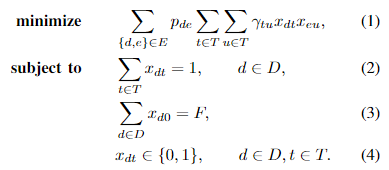
\includegraphics[width=9cm, height=3.8cm]{problem.png}


Este problema foi introduzido inicialmente por Duives~\citep{duives:13} para melhorar a distribui\c c\~ao de testes aplicados na Universidade de Bologna. A partir de seu estudo inicial foi demonstrado que o 
problema pode ser classificado como NP-Dif\'icil, e o formulou como um programa quadr\'atico bin\'ario n\~ao convexo. Em 2018, Souza~\citep{web:16} tambem abordou este mesmo problema em seu estudo utilizando heur\'isticas recombinat\'orias, seus resultados ser\~ao utilizados neste trabalho como compara\c c\~ao

\section{Estudo inicial}

Inicialmente foram implementados cinco algor\'itmos para gera\c c\~ao das solu\c c\~oes, dois deles sendo heur\'isticas construtivas, comparadas ent\~ao com duas buscas locais simples, com crit\'erio de parada de primeira melhora e melhor melhora, e por fim tambem foi implementada uma caminhada aleat\'oria para compara\c c\~ao. As abrevia\c c\~oes para os algoritmos s\~ao respectivamente H-I, H-II, BSPM, BSMM e CA.

\vspace{10pt}
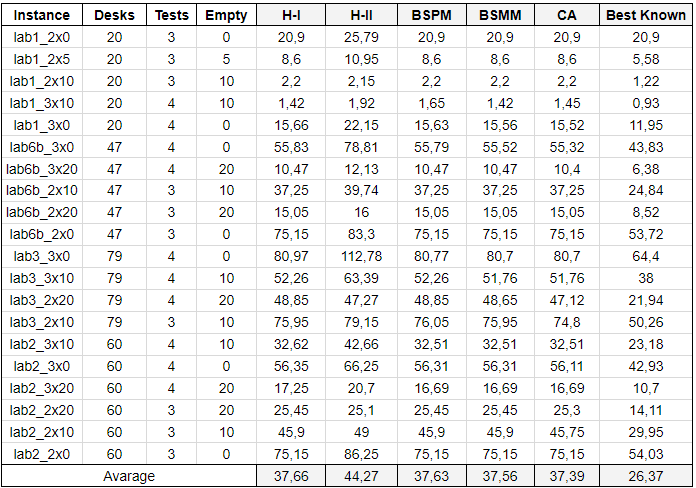
\includegraphics[width=14cm, height=10cm]{tabela 1.png}
\newline

A tabela exibe o resultado dos algoritmos citados para 20 inst\^ancias, comparando com o melhor valor conhecido para a inst\^ancia.



\section{ Implementa\c c\~ao dos algoritmos escolhidos }

Para implementa\c c\~ao foram selecionados os seguintes algoritmos: \textbf{Busca local Randomizada}, \textbf{Busca Tabu}, \textbf{Rein\'icio aleat\'orio}, \textbf{Constru\c c\~ao repetida} e \textbf{Algoritmo semi-guloso (Guloso-K)}, os mesmos foram implementados de forma a permitir reutiliza\c c\~ao / combina\c c\~ao entre eles.


\section{ Mix de abordagens }
Ap\'os a implenta\c c\~ao das abordagens anteriores nesta se\c c\~ao foram criados novos algoritmos onde misturamos mais de uma abordagem a fim de buscar uma melhor combina\c c\~ao para resolver o problema. Um exemplo de onde esta mescla pode ser ben\'efica \'e na busca tabu visto que utiliza de uma solu\c c\~ao aleat\'oria para como seu estado incial e que caso essa solu\c c\~ao inicial seja boa vinda de alguma outra abordagem a busca ter\'a a aportunidade de melhorar ainda mais este resultado. Sendo assim criamos os seguintes algoritmos: \textbf{Auto-tabu (Tabu + controle autom\'atico da \text tenure e aplica\c c\~ao de perturba\c c\~oes)}, \textbf{Tabu + Guloso-K}, \textbf{Tabu + Constru\c c\~ao repetida}, \textbf{Rein\'icio aleat\'orio + Guloso-K}, \textbf{Constru\c c\~ao repetida + Guloso-K} e \textbf{Constru\c c\~ao repetida + Perturba\c c\~ao}. 

\section{ O Algoritmo Auto-tabu}
Durante o desenvolvimento dos algoritmos, em especial na busca Tabu, notamos que em algus casos o algoritmo acabava ciclando em alguma regi\~ao da busca onde tinhamos que ficar alterando a tenure at\'e encontrar um valor de itera\c c\~oes proibidas que fazia a execu\c c\~ao sair do ciclo. O problema pode ser observado claramente no gr\'afico abaixo, onde \'e mostrada a evolu\c c\~ao do valor da fun\c c\~ao objetivo (eixo y) pelo n\'umero de itera\c c\~oes (eixo x).

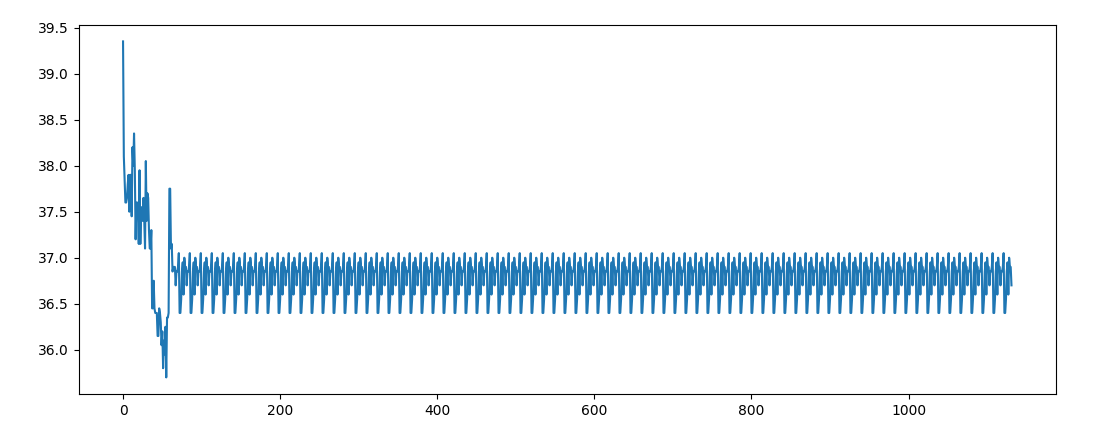
\includegraphics[width=13cm, height=10cm]{graph1.png}

A solu\c c\~ao para este problema foi inicialmente, criar uma modifica\c c\~ao no funcionamento b\'asico da busca tabu, permitindo um conjunto adicional de parametriza\c c\~oes alem da tenure, tais parametriza\c c\~oes s\~ao:

\begin{itemize}
   \item \textbf{initialTernure}: Valor inicial da "Tabu tenure"
   \item \textbf{tenureIncrement}: Incremento da Tenure a cada \textbf{cycleRange}.
   \item \textbf{cycleRange}: Ciclo (Em itera\c c\~oes) onde caso n\~ao h\'aja melhora neste per\'iodo, \'e incrementada a tenure em \textbf{tenureIncrement} unidades.
   \item \textbf{cutRange}: Altura de corte, caso a solu\c c\~ao atual ultrapasse \textbf{cutRange}\% de aumento em rela\c c\~ao a melhor conhecida, a tenure \'e zerada, a solu\c c\~ao retorna a melhor conhecida e \'e aplicada uma muta\c c\~ao aleat\'oria na mesma.
\end{itemize}

Com esta abordagem, pode-se verificar uma melhora no resultado final obtido, e tambem a elimina\c c\~ao da cliclagem que ocorria, como se verifica no gr\'afico abaixo:

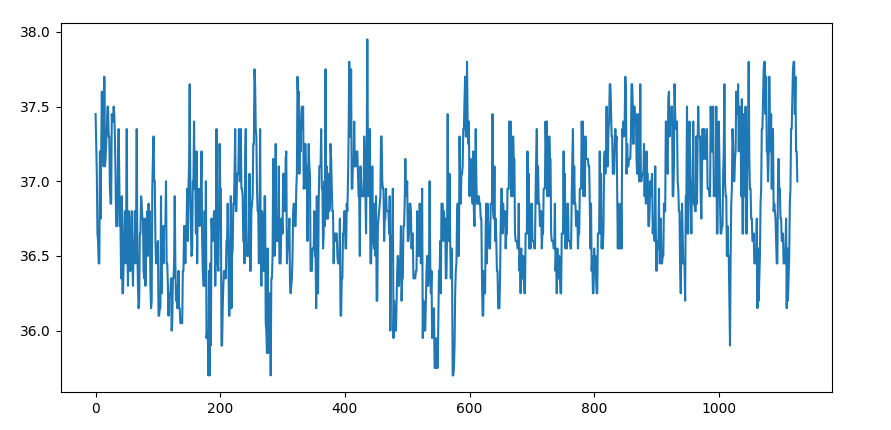
\includegraphics[width=13cm, height=10cm]{graph2.png}

Ap\'os a cria\c c\~ao dos algoritmos, foram feitos testes com cinco inst\^ancias representativas, obtendo o desvio relativo em compara\c c\~ao ao melhor resultado conhecido, os dados foram os seguintes:

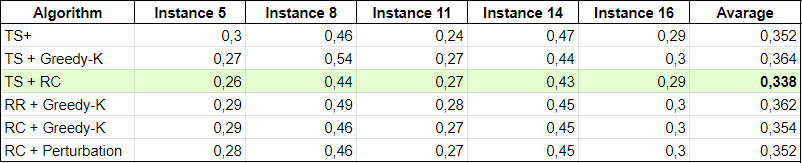
\includegraphics[width=13cm, height=3.6cm]{tabela 2.png}
\newline
Verificando os resultados, chegamos a conclus\~ao que o melhor algoritmo foi o que combina Busca Tabu com a constru\c c\~ao repetida, obtendo um desvio padr\~ao m\'edio de 0,338.


\section{ Testes finais }

Ap\'os termos definido qual o melhor algoritmo criado, fizemos uma bateria de testes com este algoritmo em todas as 20 inst\^ancias iniciais, e obtemos os seguintes resultados:

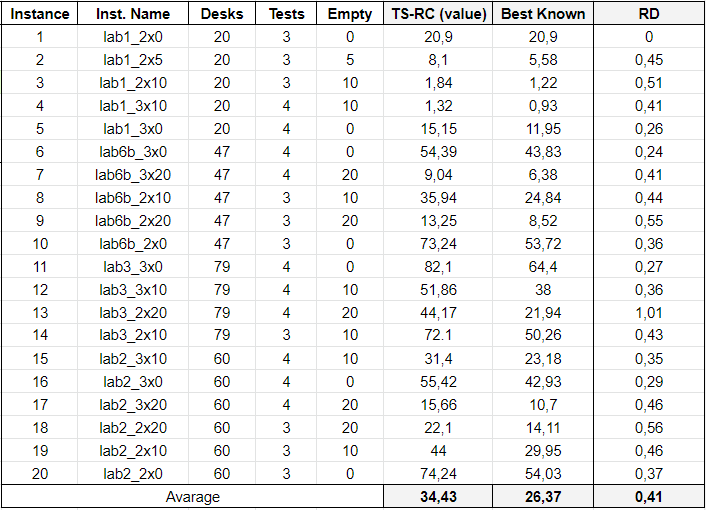
\includegraphics[width=13cm, height=10cm]{tabela 3.png}
\section{ Conclus\~ao }
Apesar de termos bons resultados durante o desenvolvimento dos algorimos h\'ibridos se comparados aos desenvolvidos inicialmente, as solu\c c\~oes obtidas ainda est\~ao um pouco longe das melhores conhecidas, j\'a que atingimos o melhor valor conhecido em apenas uma das 20 inst\^ancias selecionadas (lab1\_2x0). Verificamos que para o problema de aloca\c c\~ao de testes, a facilidade com que se aproxima das melhores solu\c c\~oes varia muito de inst\^ancia para inst\^ancia, tendo que em alguns casos, criar adapta\c c\~oes ou configura\c c\~oes para explorar regi\~oes diferentes da topologia de busca.

~\\
\bibliographystyle{sbpo}
\bibliography{exemplo-latex}


\end{document}

